% !TEX root = template.tex

\theoremstyle{definition}
\newtheorem{definition}{Definition}[section]

\theoremstyle{definition}
\newtheorem{optimization}{Optimization Problem}

\section{Introduction}

The task of analyzing large volumes of data is fairly common in the industry and has attracted a considerable amount of attention from researches. On the one hand, companies are interested in gathering every last bit of available data because this enables them to gain business-critical insight into the market. On the other hand, effective manipulation of large quantities of data is a multifaceted challenge that peaks the interest of many scholars and engineers.

Rapidly increasing amounts of data are being collected and stored on a daily basis. Some typical examples include: logs of online search queries, records of shopping-related activities on e-commerce websites, recordings of voice commands given to personal digital assistants and more. It is possible to persist all of this data because modern storage devices are as cost-effective as ever.

There is great potential for companies to improve their products and services if the collected data is used to make data-driven business decisions. However, doing analytics at scale requires algorithms and frameworks which are specifically developed for processing vast amounts of data. This paper mentions some of the most notable challenges as well as frameworks in Section~\ref{sec:related-work}. Starting with Section~\ref{sec:scheduling-algorithm}, the focus shifts to the work of \citet{Chen2017} where an algorithm for fair resource scheduling under certain restrictions is proposed.

\section{Related Work}
\label{sec:related-work}

When working with big data, it is crucial to be able to store all of it in a fault-tolerant, accessible and scalable way. The Google file system (GFS) is a rather famous distributed filesystem described in the paper by \citet{2003-ghemawat-gfs}. This filesystem is able to deliver ``high performance to a large number of clients'' and was designed to run on commodity hardware and store ``a few million of files, typically 100 MB or larger in size''. GFS design played a role in the development of the Hadoop file system (HDFS), which is one of the core components of the Apache Hadoop framework. As a file system, HDFS has proven its ability to efficiently store petabytes of data in a resilient and highly available manner. Its \href{https://wiki.apache.org/hadoop/DFS_requirements}{current design requirements could be found online\footnote{\url{https://wiki.apache.org/hadoop/DFS_requirements} (last visited \today)}} and an early description by \citet{2010-shvachko-hdfs} is available as well.

Just the ability to store vast amounts of data is not enough to be able to analyze it and extract value from it. Another notable challenge is to design suitable data processing frameworks. Such frameworks should simplify the development of data processing programs and abstract away the complexity of working with a cluster of machines. In order to achieve that, a programming model named MapReduce was proposed by \citet{2004-dean-mapreduce}. This programming model expects the data processing program (also known as a \emph{data processing job}) to be described as a pair of two functions, namely \emph{map} and \emph{reduce}. The first function transforms a key/value pair into a sequence of key/value pairs. This sequence is then consumed by the second function in such a way that the values with the same key are processed together. For example, the map function could be applied to a log file which stores different actions (such as login, password change, etc.) performed by different users of some webservice. It could then filter all log entries, leaving only the ones where the user requested a password change. The reduce function would then collect the list of times when a password change request was made by the user. The MapReduce model allows to parallelize the workload automatically, without any additional effort on the part of the programmer. One of the notable frameworks that take advantage of this model is Apache Hadoop \cite{2008-zaharia-hadoop-late}.

Although MapReduce is a profound idea, it is not always the best approach to implement a specific algorithm\footnote{\url{https://wiki.apache.org/hadoop/HadoopIsNot} (last visited \today)}. Typical examples when MapReduce fails as a computation model include machine learning algorithms that require many iterations to complete. Moreover, although Apache Hadoop has enabled the large-scale, commercial use of consumer-grade hard disk drives, it did \emph{not} do so for random access memory (RAM). In order to facilitate the use of iterative and interactive algorithms as well as speed up computations by taking advantage of the available RAM, the Apache Spark framework was developed by \citet{2016-zaharia-spark}. The core of Apache Spark is based around the concept of resilient distributed datasets (RDD) and the 2.x release of the framework introduced a Dataset API on top of it. For a proper introduction to Apache Spark a number of online tutorials as well as extensive documentation are available\footnote{\url{https://wiki.apache.org/hadoop\#Tutorials} (last visited \today)}.

When designing such frameworks for data processing, one common challenge is the fair allocation of available resources, such as computational slots, hard disk space or network bandwidth. Multiple concurrent tasks of the same data processing job compete for these resources. In addition to that, if multiple concurrent jobs run on the same cluster, they must compete with each other as well. The fair allocation of resources ensures that there is no job or user who must wait \emph{too long} in order for their data analysis to complete. More formally, the resource allocation should be \emph{max-min fair}, meaning that an attempt to redistribute the already allocated resources would result in some job or user having to wait longer than before.

The development of systems like Hadoop \cite{2008-zaharia-hadoop-late}, Spark \cite{2016-zaharia-spark}, Spanner \cite{Corbett2012}, Mesa \cite{Gupta2014}, Iridium \cite{Pu2015} or Geode \cite{Vulimiri2015} has shown that performing the computation close to where the input data is stored allows to significantly reduce the completion time of data processing jobs. In other words, it takes a lot of time to transfer large quantities of data across relatively slow networks that connect datacenters. Therefore, modern cluster resource managers, such as Hadoop Yarn or Apache Mesos, should be able to take network characteristics into account when making resource allocation decisions, especially when controlling clusters that span several georgraphically separate datacenters.

In order to minimize the completion time of an analytic job (also known as \emph{latency}), it is important to distribute the input data and corresponding tasks across several datacenters in an efficient manner. For example, the Iridium system by \citet{Pu2015} uses ``an online heuristic to redistribute the datasets \emph{prior} the queries' arrivals, and places the tasks to reduce network bottlenecks \emph{during} the query's execution''. On the other hand, the \emph{Flutter} scheduling algorithm by \citet{Hu2016} does not rely on such heuristics and instead precisely solves the scheduling problem for all tasks of a single analytic job. The exact solution is possible because the underlying optimization problem was successfully transformed into an equivalent Linear Programming (LP) problem which in turn could be efficiently solved. A generalization of the Flutter scheduling algorithm that accommodates several concurrent analytic jobs is presented by \citet{Chen2017} and outlined in the rest of this seminar paper.

\section{Scheduling Algorithm}
\label{sec:scheduling-algorithm}

\citet{Chen2017} view a data processing \emph{job} simply as a number of \emph{tasks} that comprise it. These tasks are further separated into consecutive \emph{stages}, where the future stages depend on the results of the past stages. In other words, the tasks from a single stage must wait for the tasks from all the previous stages to complete. On the contrary, within a single stage the tasks are \emph{independent} of each other and therefore could be executed in parallel.

\citet{Chen2017} further describe a geographically distributed datacenter as a group of independent datacenters connected by a network. Each single datacenter from this group contains several \emph{computing slots} which are capable of executing tasks. Furthermore, the network that connects the pairs of datacenters is expected to have significantly \emph{lower bandwidth} than the local network inside each individual datacenter. This means that transferring large amounts of data between different datacenters takes a lot of time. Finally, in order to execute a task, it must be provided with a computing slot and the necessary input data. The input data for every task is also hosted by some datacenter(s). If it so happens that a task is assigned to a datacenter that does not hold the entire input data for that task, the missing parts will be transferred across the inter-datacenter network.

\subsection{Formal Definitions}

\citet{Chen2017} define \(\mathcal{D} = \left\{1, 2, \dots, J\right\}\) to be the set whose elements are individual datacenters and the entire set itself represents one large geographically distributed datacenter. Each individual datacenter \(j\) has a limited number of computing slots denoted by \(a_j\). Furthermore, the set of analytic jobs is defined as \(\mathcal{K} = \left\{1, 2, \dots, K\right\}\). Each of the jobs \(k\) consists of a single stage which itself is a set of independent tasks \(\mathcal{T}_k=\left\{1, 2, \dots, n_k\right\}\).

In the proposed formal model the time it takes to complete a job is the \emph{longest} time one if its independent tasks takes to complete. In turn, the completion time of a task is the sum \(e^{k}_{i, j} + c^{k}_{i, j}\), where the first summand is the \emph{execution time} and the second --- \emph{network transfer time}. For both of them, index \(k\) is the analytic job, index \(i\) is the task from that job and index \(j\) is the index of the datacenter to which the task is assigned. The execution time for any possible assignment is assumed to be known in advance. The network transfer time, on the other hand, is calculated in the following fashion. Assume task \(i\) of job \(k\) requires input data that is stored by a set of individual datacenters \(S^k_i\). More specifically, for each datacenter \(s\in S^k_i\) the volume of stored input data equals to \(d^{k, s}_i\). The bandwidth between two distinct datacenters \(s\) and \(j\) is denoted by \(b_{s, j}\), where \(s\neq j\). Then the following formula computes network transfer time:

\begin{IEEEeqnarray*}{lCl}
  c^k_{i, j} &=&\left\{ \,
  \begin{IEEEeqnarraybox}[][c]{l?s}
    \IEEEstrut
    0, &  when \(S^k_i = \left\{j\right\}\),\\
    \max_{s\in S^k_i, s\neq j}\left(\frac{d^{k, s}_i}{b_{s,j}}\right) & otherwise.
    \IEEEstrut
  \end{IEEEeqnarraybox}
  \right. \\
\end{IEEEeqnarray*}

The completion time of a task depends on the datacenter which executes that task. The assignment of tasks to datacenters is captured by the indicator variables \(x^{k}_{i, j}\). More specifically, \(x^k_{i, j} = 1\) when task \(i\) of job \(k\) is assigned to datacenter \(j\), and otherwise \(x^k_{i, j} = 0\). This leads to the following formula for the completion time of the entire job \(k\):

\[\tau_k = \max_{i\in\mathcal{T}_k, j\in\mathcal{D}}x^k_{i, j}\left(e^k_{i, j} + c^k_{i, j}\right).\]

\subsection{Optimization Problem}

\citet{Chen2017} introduce the following definitions which are later used to formulate the optimization problem:

\newcommand{\flvr}{\langle\mathbf{v}\rangle}
\newcommand{\fbma}{\mathbf{\alpha}}
\newcommand{\flar}{\langle\fbma\rangle}
\newcommand{\fbmb}{\mathbf{\beta}}
\newcommand{\flbr}{\langle\fbmb\rangle}

\begin{definition}[Non-increasingly sorted \(\flvr\)]
  \label{def:def1}
  Let \(\flvr_k\) denote the \(k\)-th (\(1\leq k \leq K\)) largest element of \(\mathbf{v}\in\mathbb{Z}^K\), implying \(\flvr_1\geq\flvr_2\geq\ldots\geq\flvr_K\). Then \(\mathbf{\flvr} = \left(\flvr_1, \flvr_2, \dots, \flvr_K\right)\) represents the non-increasingly sorted version of \(\mathbf{v}\).
\end{definition}
\begin{definition}[Lexicographically smaller vector]
  For any \(\fbma\in\mathbb{Z}^K, \fbmb\in\mathbb{Z}^K\), if \(\flar_1\leq\flbr_1\) or \(\exists k\in \left\{1,2,\dots, K\right\}\) s.t. \(\flar_k\leq\flbr_k\) and \(\flar_i = \flbr_i, \forall i\in [1, \dots, k)\), then \(\fbma\) is lexicographically smaller than \(\fbmb\), denoted \(\fbma \preceq \fbmb\).
\end{definition}
\begin{definition}[Lexicographic minimization]
  Lexicographic minimization of vector \(\mathbf{f}\) is represented with \(\text{lexmin}_{\mathbf{x}}\mathbf{f}\) with the optimal solution \(\mathbf{x^*}\in\mathbb{R}^K\) s.t. \(\forall \mathbf{x}\in\mathbb{R}^K: \mathbf{f}(\mathbf{x^*})\preceq\mathbf{f}(\mathbf{x})\)
\end{definition}

With the above definitions in place, the following optimization problem is formulated:

\newcommand{\foralltdk}{\forall i \in \mathcal{T}_k, \forall j\in\mathcal{D}, \forall k\in\mathcal{K}}
\newcommand{\fcapacity}{\sum_{k\in\mathcal{K}}\sum_{i\in\mathcal{T}_k} x^k_{i, j} \leq a_j}
\newcommand{\fcapacityq}{\forall j\in\mathcal{D}}
\newcommand{\fpresence}{\sum_{j\in\mathcal{D}}x^k_{i, j} = 1}
\newcommand{\fpresenceq}{\forall i\in\mathcal{T}_k, \forall k\in\mathcal{K}}

\begin{optimization}
  \label{opt:opt1}
  \begin{IEEEeqnarray}{lrCll}
    \text{lexmin}_{\mathbf{x}} & \mathbf{f} &=&\left(\tau_1, \tau_2, \dots, \tau_K\right) \label{eq:cost}&\\
    \text{s.t.} & \tau_k &=& \max_{i\in\mathcal{T}_k, j\in\mathcal{D}} x^k_{i, j}\left(c^k_{i, j} + e^k_{i, j}\right), &\forall k\in\mathcal{K} \label{eq:goal}\\
    &&& \fcapacity,  &\fcapacityq\label{eq:capacity}\\
    &&& \fpresence,  &\fpresenceq\label{eq:presence}\\
    &&& x^k_{i, j} \in \left\{0, 1\right\}. &\foralltdk\label{eq:onehot}
  \end{IEEEeqnarray}
\end{optimization}

Optimization Problem~\ref{opt:opt1} begins by choosing an assignment of tasks to datacenters. This assignment is captured by the values of \(x^k_{i, j}\) and must satisfy constraints \eqref{eq:capacity}, \eqref{eq:presence} and \eqref{eq:onehot}. In particular, constraint \eqref{eq:capacity} ensures that every datacenter is not assigned more tasks than the number of its available computing slots. Constraint \eqref{eq:presence} guarantees that each task is assigned to exactly one datacenter. Finally, constraint \eqref{eq:onehot} captures the fact that \(x^k_{i, j}\) is an indicator variable which is equal to one if and only if task \(i\) from job \(k\) is assigned to datacenter \(j\). Once these constraints are satisfied, constraint \eqref{eq:goal} shows how to compute the completion time of the analytic job \(k\). Finally, the cost function \eqref{eq:cost} is an instance of lexicographic minimization which collects the computed job completion times into a vector. The coordinates of this vector are ordered by value from largest to smallest. By repeatedly choosing assignments that satisfy the constraints, several such vectors are produced. By choosing the lexicographically smallest vector, it is guaranteed that the largest job completion time is not larger than that from all the other vectors. Among all of the vectors with the same largest job completion time, the vector with the smallest second-largest job completion time is chosen, and so on. This means that the solution to the Optimization Problem~\ref{opt:opt1} is an assignment of tasks to datacenters that minimizes job completion times in a max-min fair fashion.

Unfortunately, there are several factors that make Optimization Problem~\ref{opt:opt1} difficult to solve, as pointed out by \citet{Chen2017}:

\begin{enumerate}
\item The cost function is multi-objective.
\item Constraint \eqref{eq:goal} is not linear.
\item Constraint \eqref{eq:onehot} is integral.
\end{enumerate}

These factors are eliminated by a sequence of transformations. Optimization Problem~\ref{opt:opt2} replaces the multi-objective cost function with a single-objective one. However, this transformation slightly changes the meaning of the underlying optimization problem: only the largest job completion time is now being minimized. As it later turns out, the solution of Optimization Problem~\ref{opt:opt2} could be used to restore the solution of the initial Optimization Problem~\ref{opt:opt1}.

\begin{optimization}
  \label{opt:opt2}
  \begin{IEEEeqnarray}{ll}
    \min_{\mathbf{x}} & \quad \max_{k\in\mathcal{K}}\left(\tau_k\right) \\
    \text{s.t.}  & \quad \text{Constraints \eqref{eq:goal}, \eqref{eq:capacity}, \eqref{eq:presence} and \eqref{eq:onehot} hold.}
  \end{IEEEeqnarray}
\end{optimization}

Optimization Problem~\ref{opt:opt3} eliminates the non-linear constraint \eqref{eq:goal}. This is achieved by simply substituting \(\tau_k\) in the cost function with the non-linear equation that computes it:

\begin{optimization}
  \label{opt:opt3}
  \begin{IEEEeqnarray}{ll}
    \min_{\mathbf{x}} & \quad \max_{k\in\mathcal{K}}\left(\max_{i\in\mathcal{T}_k, j\in\mathcal{D}} x^k_{i, j}\left(c^k_{i, j} + e^k_{i, j}\right)\right) \\
    \text{s.t.}  & \quad \text{Constraints \eqref{eq:capacity}, \eqref{eq:presence} and \eqref{eq:onehot} hold.}
  \end{IEEEeqnarray}
\end{optimization}

At this point it remains to remove the integer constraints \eqref{eq:onehot}. \citet{Chen2017} successfully do so by proving that Optimization Problem~\ref{opt:opt3} actually belongs to a class of optimization problems described by \citet{Meyer1976}. For this class of optimization problems a reduction to an equivalent Linear Programming (LP) problem is possible. The exact conditions describing the class as well as the \(\lambda\)-technique to reduce to an LP problem is presented by \citet{Meyer1976}.

\subsection{Proposed Scheduling Algorithm}

Having shown that Optimization Problem~\ref{opt:opt3} could be reduced to an equivalent LP problem, \citet{Chen2017} propose the following scheduling algorithm:

\begin{algorithm}[H]
  \label{alg:main}
  \SetKwInOut{Input}{Input}
  \SetKwInOut{Output}{Output}
  \Input{Input data distribution \(d^{k, s}_i\), bandwidth between pairs of datacenters \(b_{s, j}\), execution time \(e_{i, j}^k\), datacenter capacities \(a_j\)}
  \Output{Task assignment \(x_{i, j}^k\)}

  Initialize \(\mathcal{K}' = \mathcal{K}\) \\
  \While{\(\mathcal{K}' \neq \emptyset\)} {
    Solve the tractable LP problem, obtain assignment \(\mathbf{x}\) \\
    Find largest completion time: \[x_{i^*, j^*}^{k^*} = \argmax\limits_{x_{i, j}^k \in\mathbf{x}} x_{i, j}^k\left(e^k_{i, j} + c^k_{i, j}\right)\] \\
    Fix \(x_{i^*, j}^{k^*},\forall j\in\mathcal{D}\); Remove them from \(\mathbf{x}\) \\
    Reduce resource capacity of the corresponding datacenter \\
    Set \(\phi\left(x^{k^*}_{i, j}\right) = x^{k^*}_{i, j}\left(c^{k^*}_{i^*, j^*} + e^{k^*}_{i^*, j^*}\right),\forall i\in \mathcal{T}_{k^*}, \forall j\in \mathcal{D}\) \\
    Remove \(k^*\) from \(\mathcal{K}'\)
  }
  \caption{Scheduling algorithm that iteratively solves the equivalent LP}
\end{algorithm}

The proposed Algorithm~\ref{alg:main} requires information about the geographically distributed datacenter in the form of individual datacenter capacities \(a_j\) as well as bandwidth characteristics \(b_{s, j}\) between each pair of datacenters \(s\neq j\). Together with the distribution of input data \(d^{k, s}_i\) and task execution times \(e_{i, j}\) this is enough information to formulate Optimization Problem~\ref{opt:opt3}, reduce it to the equivalent LP problem and solve this LP problem. On each iteration, the solution to the LP problem is an assignment of tasks to datacenters which minimizes the completion time of the longest analytic job. In other words, it produces a job \(k^*\) whose longest task \(i^*\) runs in datacenter \(j^*\). At this point, the assignment \(x^{k^*}_{i^*, j^*} = 1\) becomes fixed. Even further, indicator variables related to the same task become fixed as well: \(x^{k^*}_{i^*, j}=0, \forall j\in\mathcal{D}\setminus \left\{j^*\right\}\). The number of available computing slots of datacenter \(j^*\) must be decreased by one too. Finally, although the completion time of the entire job \(k^*\) is already known, its tasks \(i\neq i^*\) do not have a fixed assignment to their datacenters yet. However, since any such assignment will not change the completion time of the analytic job \(k^*\), the completion time of all the tasks \(i\neq i^*\) from that job is set to the completion time of that job. This ensures that during the next iteration of Algorithm~\ref{alg:main} a \emph{different} data processing job will be chosen.

\section{Evaluation of the Scheduling Algorithm}

\citet{Chen2017} evaluate their scheduling algorithm in the Apache Spark framework \cite{Zaharia2012}. Apache Spark is an open source, fault-tolerant cluster computing system that is able to perform iterative processing of analytic jobs at scale. It was initially created in 2009 at the University of California at Berkeley and then donated to the Apache Software Foundation in 2013. Notably, it was the most active Apache Software top-level project in 2014 \footnote{\url{https://blogs.apache.org/foundation/entry/the_apache_software_foundation_announces50} (last visited \today)}.

\subsection{Experimental Setup}

\begin{figure}
  \centering
  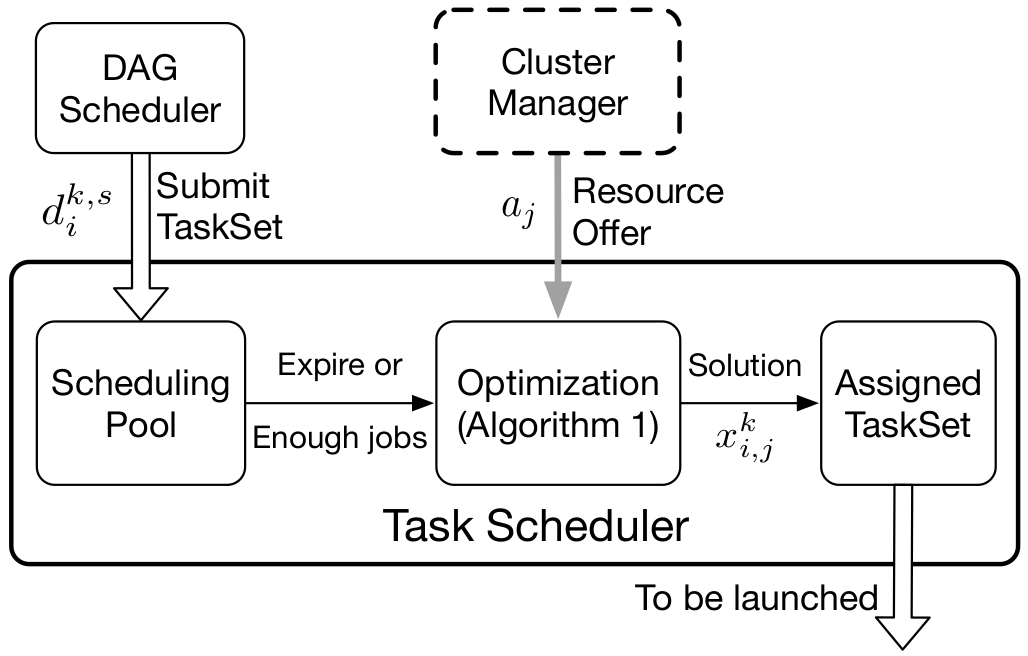
\includegraphics[width=0.6\textwidth]{architecture} \\
  \caption{Implementation of the scheduling algorithm in Spark by \citet{Chen2017}.}
  \label{fig:architecture}
\end{figure}

As illustrated by \autoref{fig:architecture}, \citet{Chen2017} substituted a component of the Apache Spark framework called \texttt{TaskScheduler} with their own implementation that incorporates Algorithm~\ref{alg:main}. Then they tested their scheduler on a cluster of \emph{twelve} virtual machines located in \emph{six} different datacenters, with \emph{two} machines per datacenter. The Apache Spark cluster was configured to run in standalone mode with no external resource manager and no database. The legacy \texttt{Sort} application was used as the benchmark workload. \citet{Chen2017} argued that, despite this being a rather simple analytic job with only two stages, the \texttt{Sort} job usually generates a fair amount of traffic between cluster nodes. This would be sufficient to test whether the proposed scheduling algorithm properly minimizes job completion times and takes into account the data transfer.

In total, three scenarios with \emph{three}, \emph{four} and \emph{five} concurrent \texttt{Sort} jobs were performed. The first \emph{two} scenarios were configured to run each job with \emph{three} parallel tasks. The last scenario with the \emph{five} jobs was configured in such a way as to have \emph{twelve} tasks in total, which is equal to the number of available nodes in the cluster. Each task operated on a 100 MB dataset with 10,000 key-value pairs. The completion times were compared against the results achieved with the default scheduling of Spark in standalone mode. An example distribution of input data as well as inter-datacenter network speeds are shown in \autoref{fig:alloc}. In particular, \autoref{fig:alloc} shows that there were 4 data processing jobs A, B, C and D each of which consisted of three tasks (e.g. A1, A2 and A3). Each task was scheduled in one of the six datacenters which are depicted as circles. The datacenters are pairwise connected, with connection speeds shown in megabits per second.

\begin{figure}
  \centering
  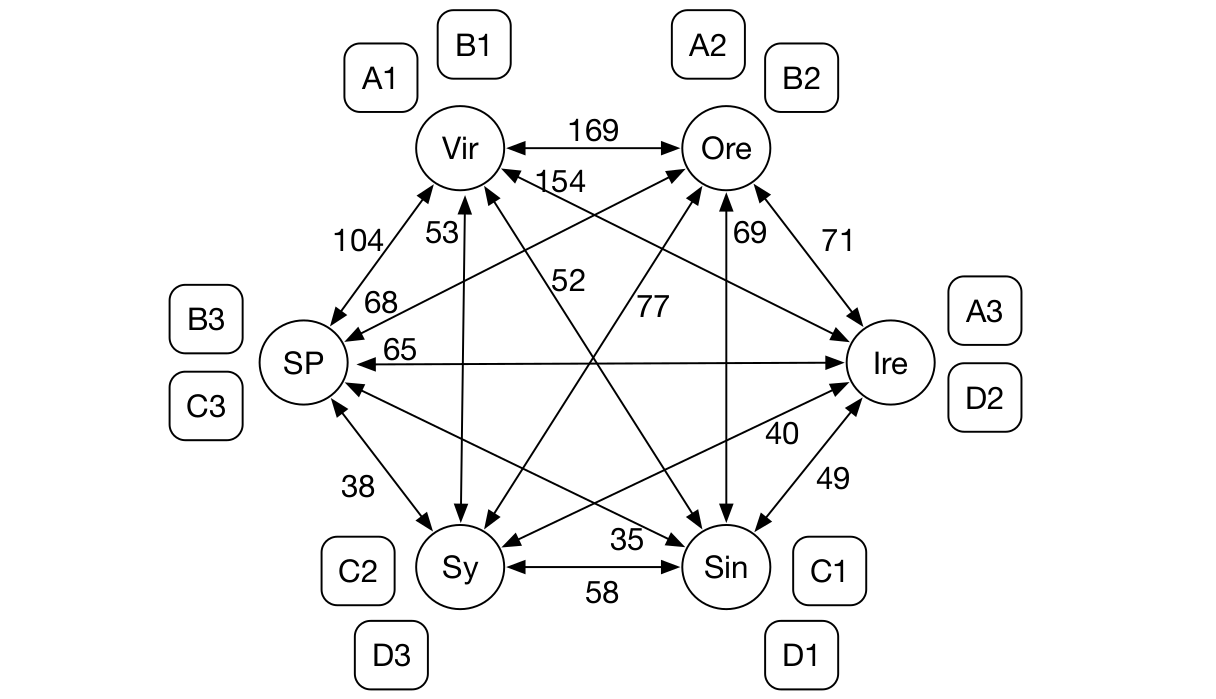
\includegraphics[width=0.8\textwidth]{alloc} \\
  \caption{Example allocation of tasks and input data by \citet{Chen2017}.}
  \label{fig:alloc}
\end{figure}

\subsection{Experimental Results}

The results of the comparison are summarized by \autoref{fig:main_result}. The top row contains the worst completion times and the bottom row contains the second-worst ones (averaged across \emph{ten} runs). Higher values correspond to longer completion times. The dashed line is the default Spark scheduler while the solid line is the proposed scheduling algorithm. As could be seen from the top row of \autoref{fig:main_result}, the proposed scheduling algorithm performed better than the default one, meaning that the completion times of the longest-running jobs are smaller. This property is actually guaranteed by Algorithm~\ref{alg:main}. The proposed algorithm also showed lower second-worst completion times, where there is no such theoretical guarantee. This fact is captured by the bottom row of \autoref{fig:main_result}.

\begin{figure}
  \centering
  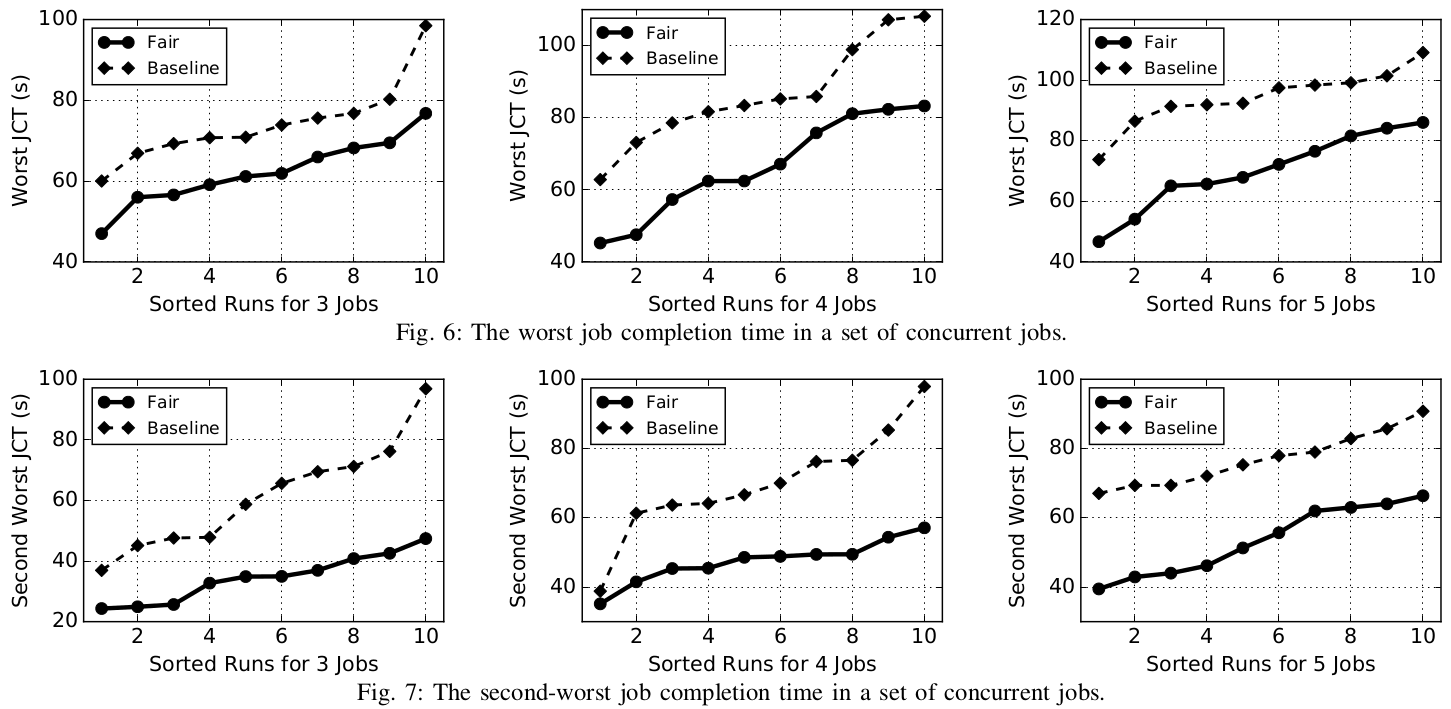
\includegraphics[width=\textwidth]{main_result} \\
  \caption{Summary of experimental results by \citet{Chen2017}.}
  \label{fig:main_result}
\end{figure}

The time to execute Algorithm~\ref{alg:main} was also measured during the experiments and is shown in \autoref{fig:algo_time}. The horizonal axis is the number of indicator variables \(x^k_{i, j}\) contained in the equivalent LP problem. Recall that the cluster consists of twelve computing slots (i.e. six datacenters with two computing slots each). Then the first bin of the histogram plot in \autoref{fig:algo_time} shows the time it takes to assign one task to some node in the cluster. In contrast, the last bin in \autoref{fig:algo_time} shows the time it takes to assign ten such tasks. This shows that the scheduling algorithm is reasonably fast and capable of scheduling a handful of tasks in a matter of seconds.

\begin{figure}
  \centering
  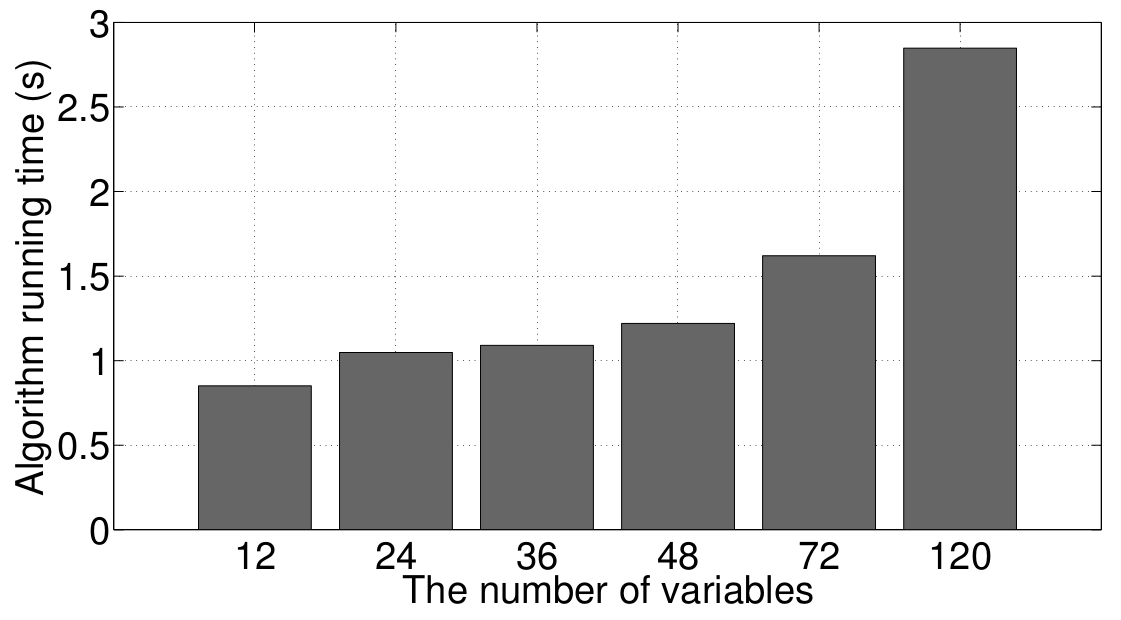
\includegraphics[width=0.6\textwidth]{algo_time} \\
  \caption{Scheduling algorithm running times by \citet{Chen2017}.}
  \label{fig:algo_time}
\end{figure}

\section{Summary}

\citet{Chen2017} describe the problem of running several competing data processing jobs on a geographically distributed cluster of nodes. They formulate and solve the optimization problem that minimizes the longest completion time of several parallel analytic jobs. The resulting scheduling algorithm takes into account that the input data is stored across a geographically distributed datacenter and allocates the limited available computing slots in a max-min fair fashion. The achieved job completion times are shorter than those of the default Apache Spark scheduler on the suggested benchmark. This result is largely due to the fact that the optimization problem and the resulting scheduling algorithm account for network transfer speeds between the geographically distributed datacenters.
